% 1.1
\subsection{Image Point Selection and Coordinates}
We manually selected the ten image coordinates $(u_i,v_i)$ corresponding to the cardinal points of the house in \texttt{house1.png} and \texttt{house2.png}. Table~\ref{tab:imgpts2} lists the points for \texttt{house1.png}, and the points for \texttt{house2.png}.

\begin{table}[H]
  \centering
  \begin{tabular}{c|cc}
    $i$ & $u_i$ & $v_i$ \\
    \hline
    1 & 285.0 & 408.0 \\
    2 & 414.0 & 267.0 \\
    3 & 483.0 & 274.0 \\
    4 & 609.0 & 61.0  \\
    5 & 750.0 & 215.0 \\
    6 & 575.0 & 482.0 \\
    7 & 411.0 & 58.0  \\
    8 & 680.0 & 337.0 \\
    9 & 277.0 & 245.0 \\
    10 & 734.0 & 393.0\\
\end{tabular}
\hspace{2cm}
\begin{tabular}{c|cc}
    $i$ & $u_i$ & $v_i$ \\
    \hline
    1 & 286.0 & 444.0 \\
    2 & 343.0 & 287.0 \\
    3 & 377.0 & 292.0 \\
    4 & 689.0 & 73.0  \\
    5 & 807.0 & 249.0 \\
    6 & 384.0 & 536.0 \\
    7 & 340.0 & 57.0  \\
    8 & 662.0 & 392.0 \\
    9 & 283.0 & 269.0 \\
    10 & 793.0 & 480.0\\
\end{tabular}
\caption{Image coordinates for \texttt{house2.png} and \texttt{house2.png}}
\label{tab:imgpts2}
\end{table}

% 1.2
\subsection{Projection Matrix Estimation via DLT}
Following the Direct Linear Transform (DLT) algorithm, we assembled the homogeneous system $A\mathbf{p}=0$ from the world coordinates $\mathbf{X}_i$ (given in \texttt{coords.tex}) and the image points. Solving by SVD gave the projection matrices:

\[
P_1 = \begin{pmatrix}
-0.137859 & -0.203597 & 0.013123 & -0.742593 \\
 0.006457 & -0.010256 & 0.235090 & -0.576638 \\
 0.000099 & -0.000136 & 0.00002853 & -0.001440
\end{pmatrix}
\]
\[
P_2 = \begin{pmatrix}
-0.022210 & -0.265996 & 0.003833 & -0.696883 \\
 0.033914 & -0.015285 & 0.251539 & -0.615171 \\
 0.000169 & -0.000077 & 0.00000740 & -0.001334
\end{pmatrix}.
\]


\begin{figure}[H]
  \centering
  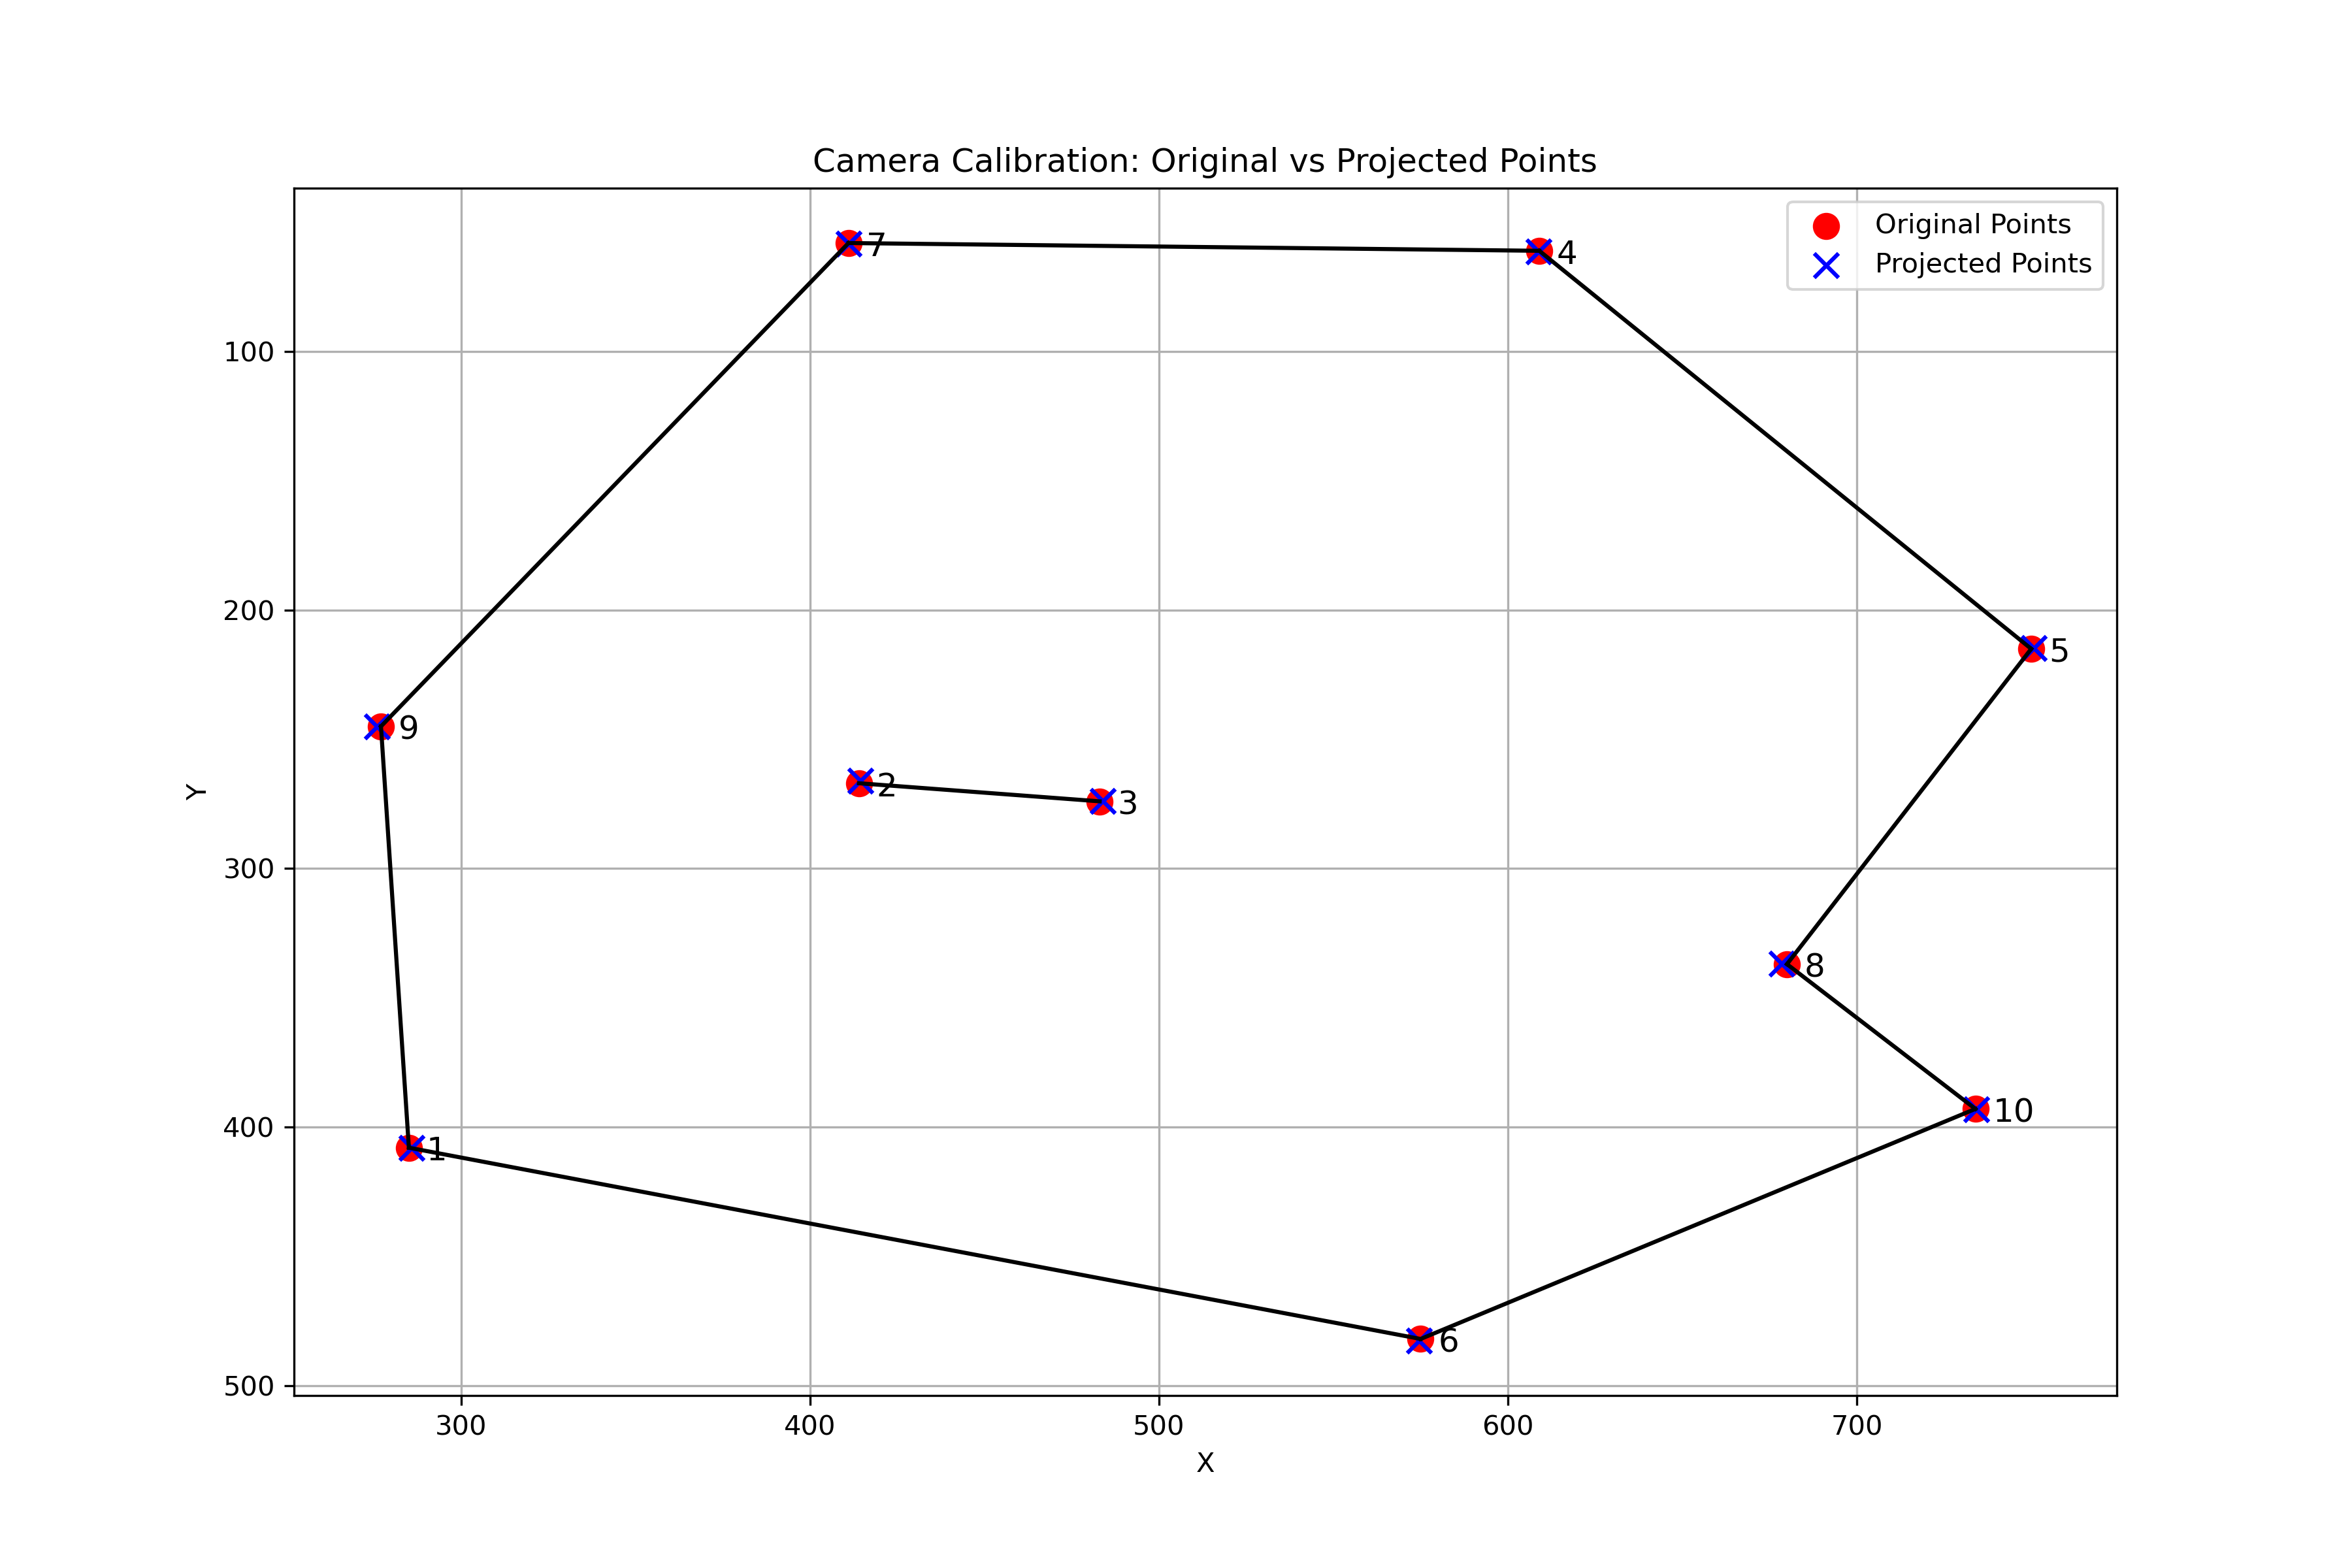
\includegraphics[width=0.4\textwidth]{"../Assets/img1.png"}
  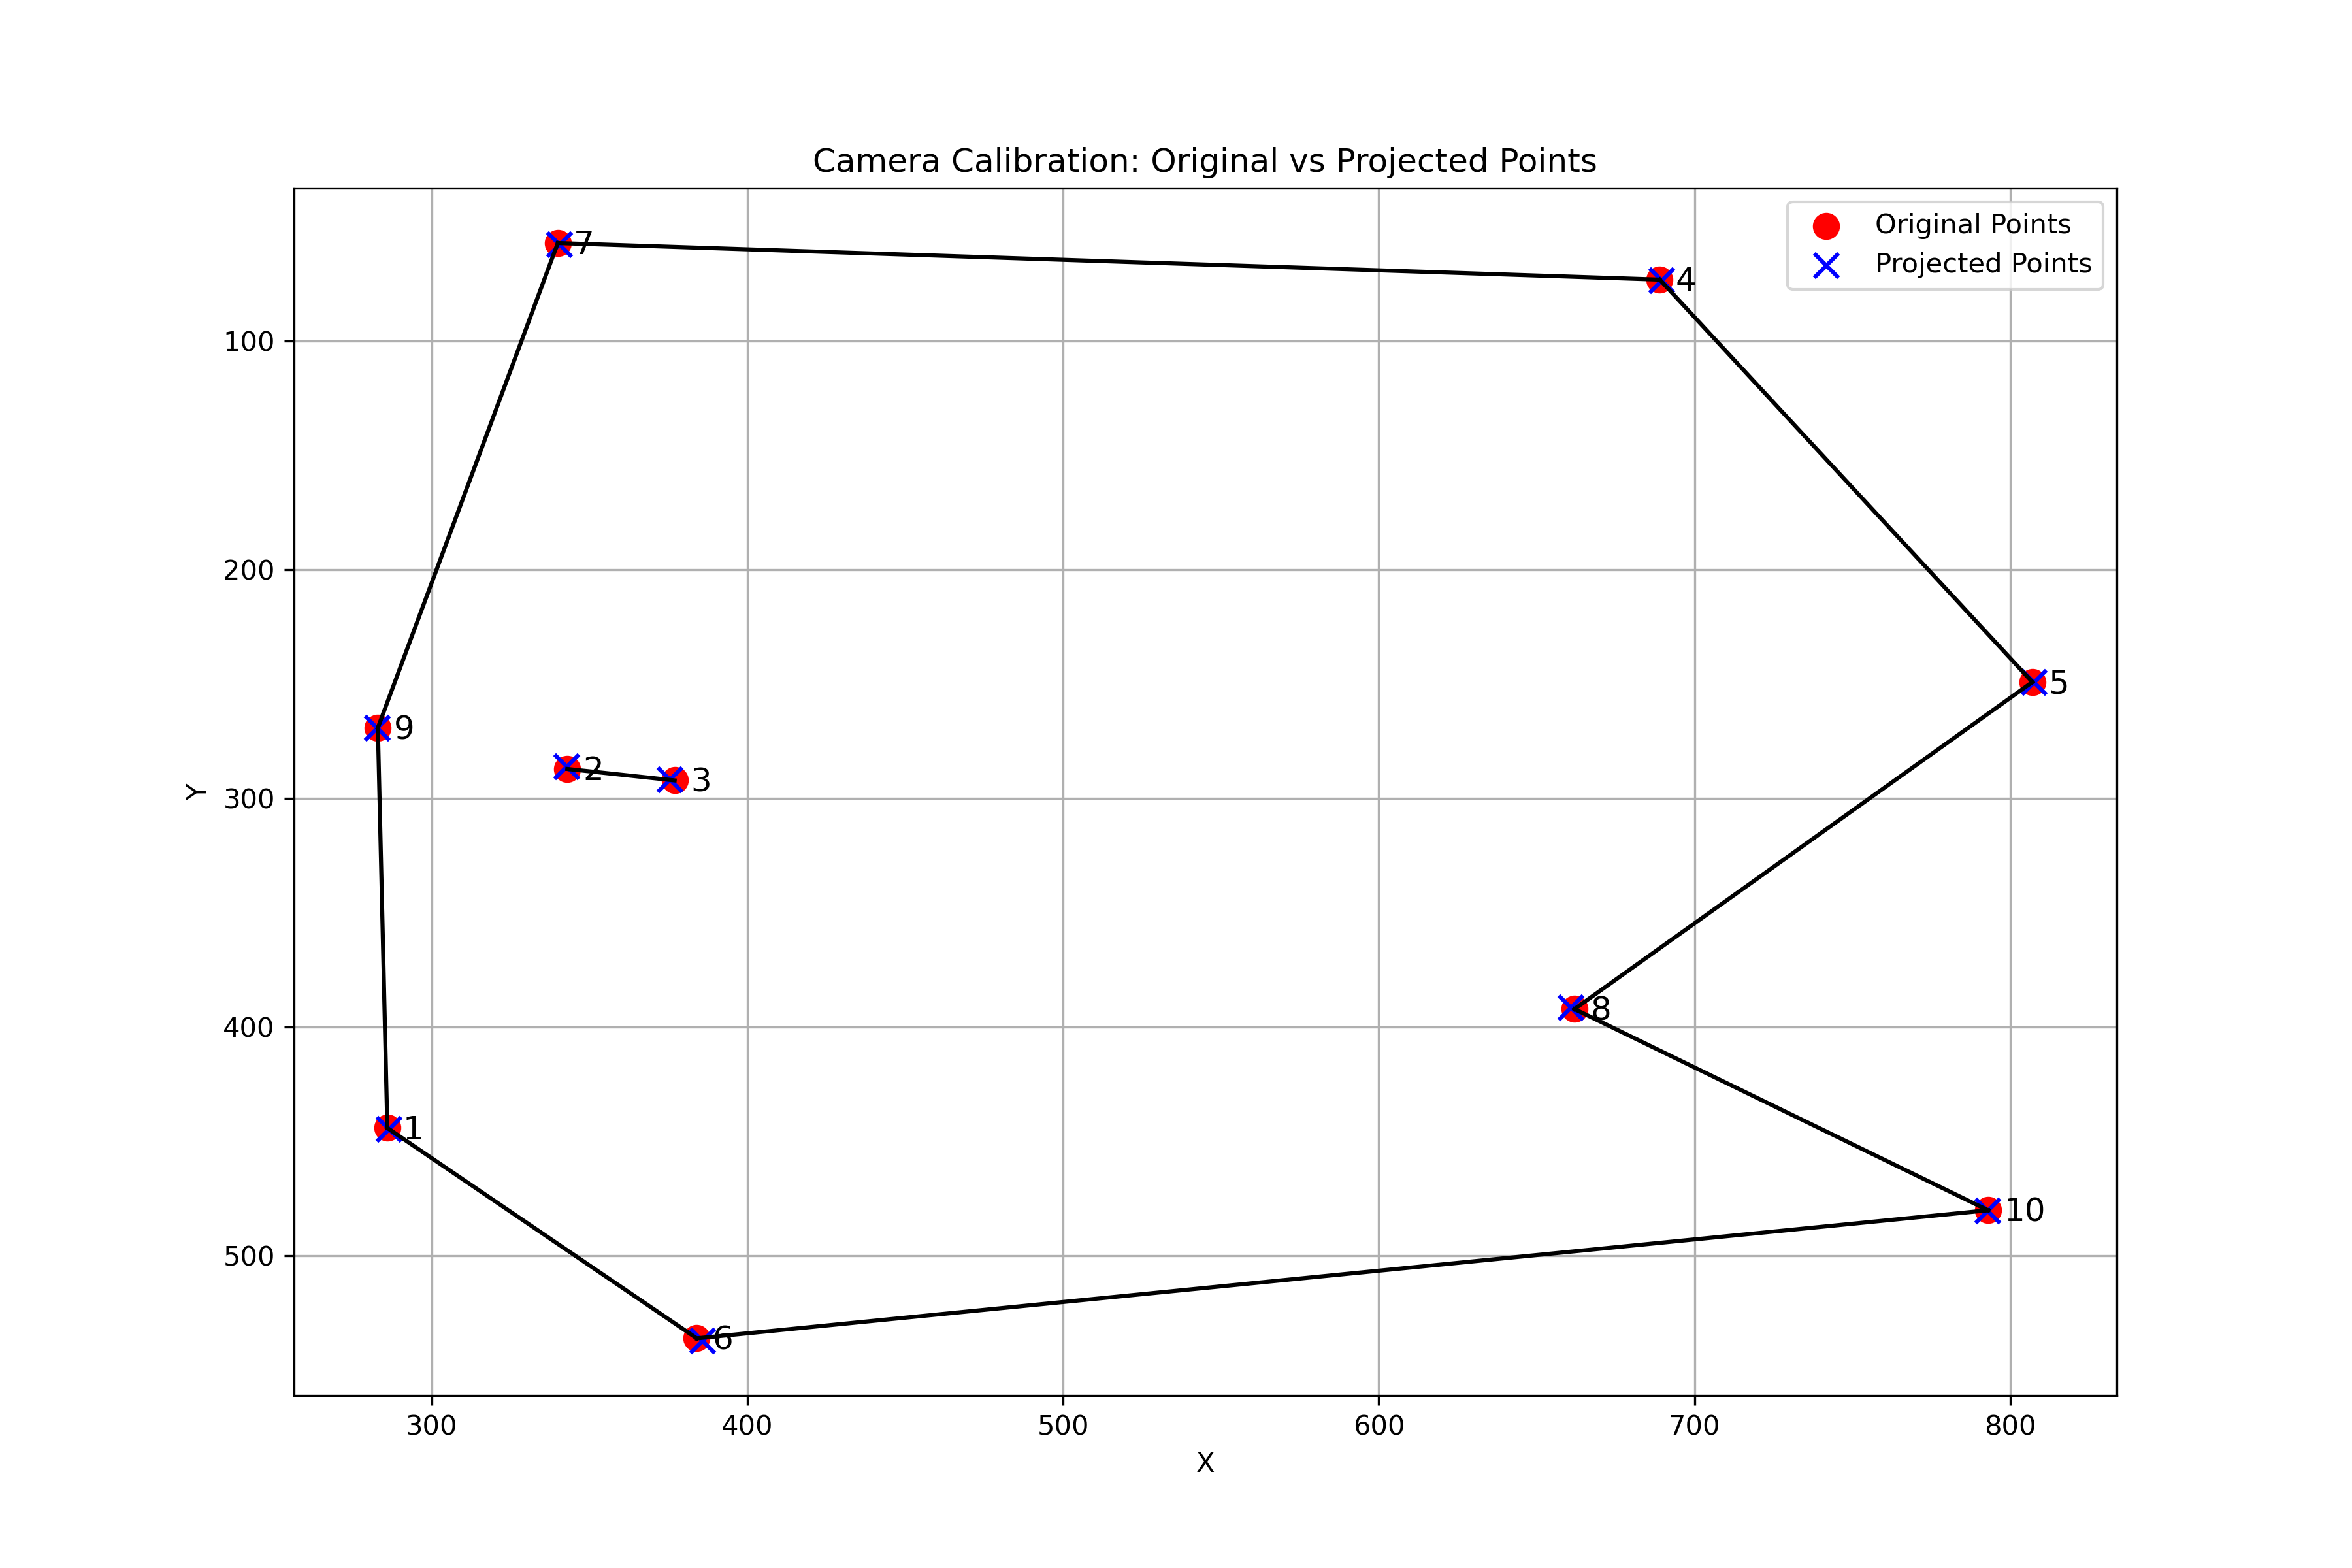
\includegraphics[width=0.4\textwidth]{"../Assets/img2.png"}
  \caption{Reprojection of the points using the estimated projection matrices for house1 and house2.}
  \label{fig:reproj}
\end{figure}

% 1.3
\subsection{Intrinsic and Extrinsic Parameter Recovery}
Decomposing each $P_j$ by RQ decomposition of its left $3\times3$ submatrix yields the intrinsic matrix $K_j$, rotation matrix $R_j$, and camera center $\tilde C_j$. The results are:

\[
K_1 = \begin{pmatrix}
1356.21 & 0.561 & 492.43 \\
0 & 1346.33 & 300.18 \\
0 & 0 & 1
\end{pmatrix},
\quad
R_1 = \begin{pmatrix}
-0.8069 & -0.5906 & 0.0036 \\
-0.1016 & 0.1328 & -0.9859 \\
 0.5818 & -0.7959 & -0.1672
\end{pmatrix},
\]
\[
\tilde C_1 = (4.7285,\,-6.7183,\,2.0299)^T.
\]

\[
K_2 = \begin{pmatrix}
1351.75 & -0.4345 & 485.33 \\
0 & 1344.28 & 253.88 \\
0 & 0 & 1
\end{pmatrix},
\quad
R_2 = \begin{pmatrix}
-0.4148 & -0.9099 & -0.0006 \\
-0.0360 & 0.0171 & -0.9992 \\
 0.9092 & -0.4145 & -0.0398
\end{pmatrix},
\]
\[
\tilde C_2 = (6.4066,\,-3.1348,\,1.3914)^T.
\]
The average reprojection errors are 0.79\,px for image 1 and 0.93\,px for image 2, indicating subpixel accuracy.